\chapter{Auenland DNS}
Ein DNS-Server im "Auenland"-Netz mit der IP-Adresse \url{	10.0.68.110}. \\

\cvss{av=local, ac=low, pr=none, ui=required, s=changed, c=high, i=low, a=low}
\cvssdescription{Brute-Force-Angriff auf den SSH-Login des DNS-Servers mit bekannten Nutzernamen und einer Passwortliste.}

\section{\makecvssbadge Auenland DNS-Server: Bruteforce}
\cvssaddtosummary{Auenland DNS-Server: Bruteforce}
\subsection*{Proof of concept}
Durch die Kompromittierung des Nextcloud-Servers konnte herausgefunden werden, dass der DNS-Server "Auenland" durch den Benutzer \textit{pippin} administriert wird. Daher wurde ein Brute-Force-Angriff auf das SSH-Login des DNS-Servers durchgeführt. Als Benutzernamen wurden \textit{admin} und \textit{pippin}gewählt und für die Passwörter wurde eine Passwortliste verwendet. Durch diesen Brute-Force-Angriff war es möglich, die gültigen Credentials für den Benutzer \textit{pippin} zu erlangen und sich mit diesem per SSH auf dem DNS-Server zu verbinden. Ein Beweis dafür ist in \autoref{fig:10_dns_proof} zu sehen.\\

\begin{figure}[!ht]
    \centering
    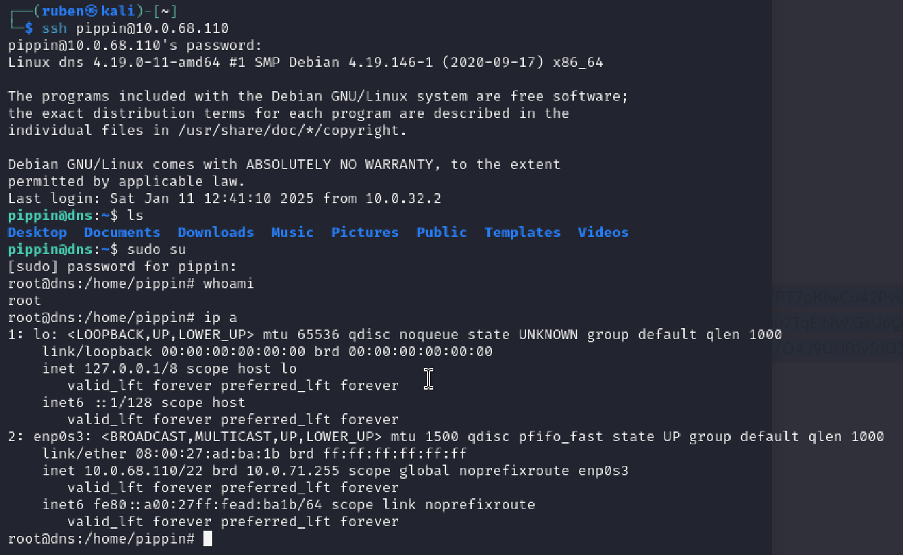
\includegraphics[width=\linewidth]{images/proofs/10_dns_proof.png}
    \caption{Proof für den DNS Server Auenland}
    \label{fig:10_dns_proof}
\end{figure}

\subsection*{Empfehlungen}
\begin{itemize}
    \item Starke Passwort-Richtlinien: Erzwingen Sie komplexe, lange Passwörter und ändern Sie Standardpasswörter, um einfache Passwörter zu vermeiden.
    \item Account-Sperrung und Rate Limiting: Implementieren Sie Mechanismen, die nach mehreren fehlgeschlagenen Login-Versuchen eine Sperrung oder Verzögerung auslösen, um automatisierte Angriffe zu behindern.
    \item Multi-Faktor-Authentifizierung (MFA): Ergänzen Sie die Passwortauthentifizierung mit einem zusätzlichen Faktor, um den Zugriff auch bei kompromittierten Zugangsdaten zu verhindern.
\end{itemize}